\section{Erdbeben}
\label{sec:erdbeben}

Erdbeben sind geophysikalische Extremereignisse, die eine Erschütterung des Erdkörpers darstellen und meist durch tektonische Massenverschiebungen an den Bruchfugen der Platten in der Lithosphäre, aber auch durch vulkanische Aktivität ausgelöst werden. \cite{ETHZ}

\begin{figure}[ht]
    \centering
    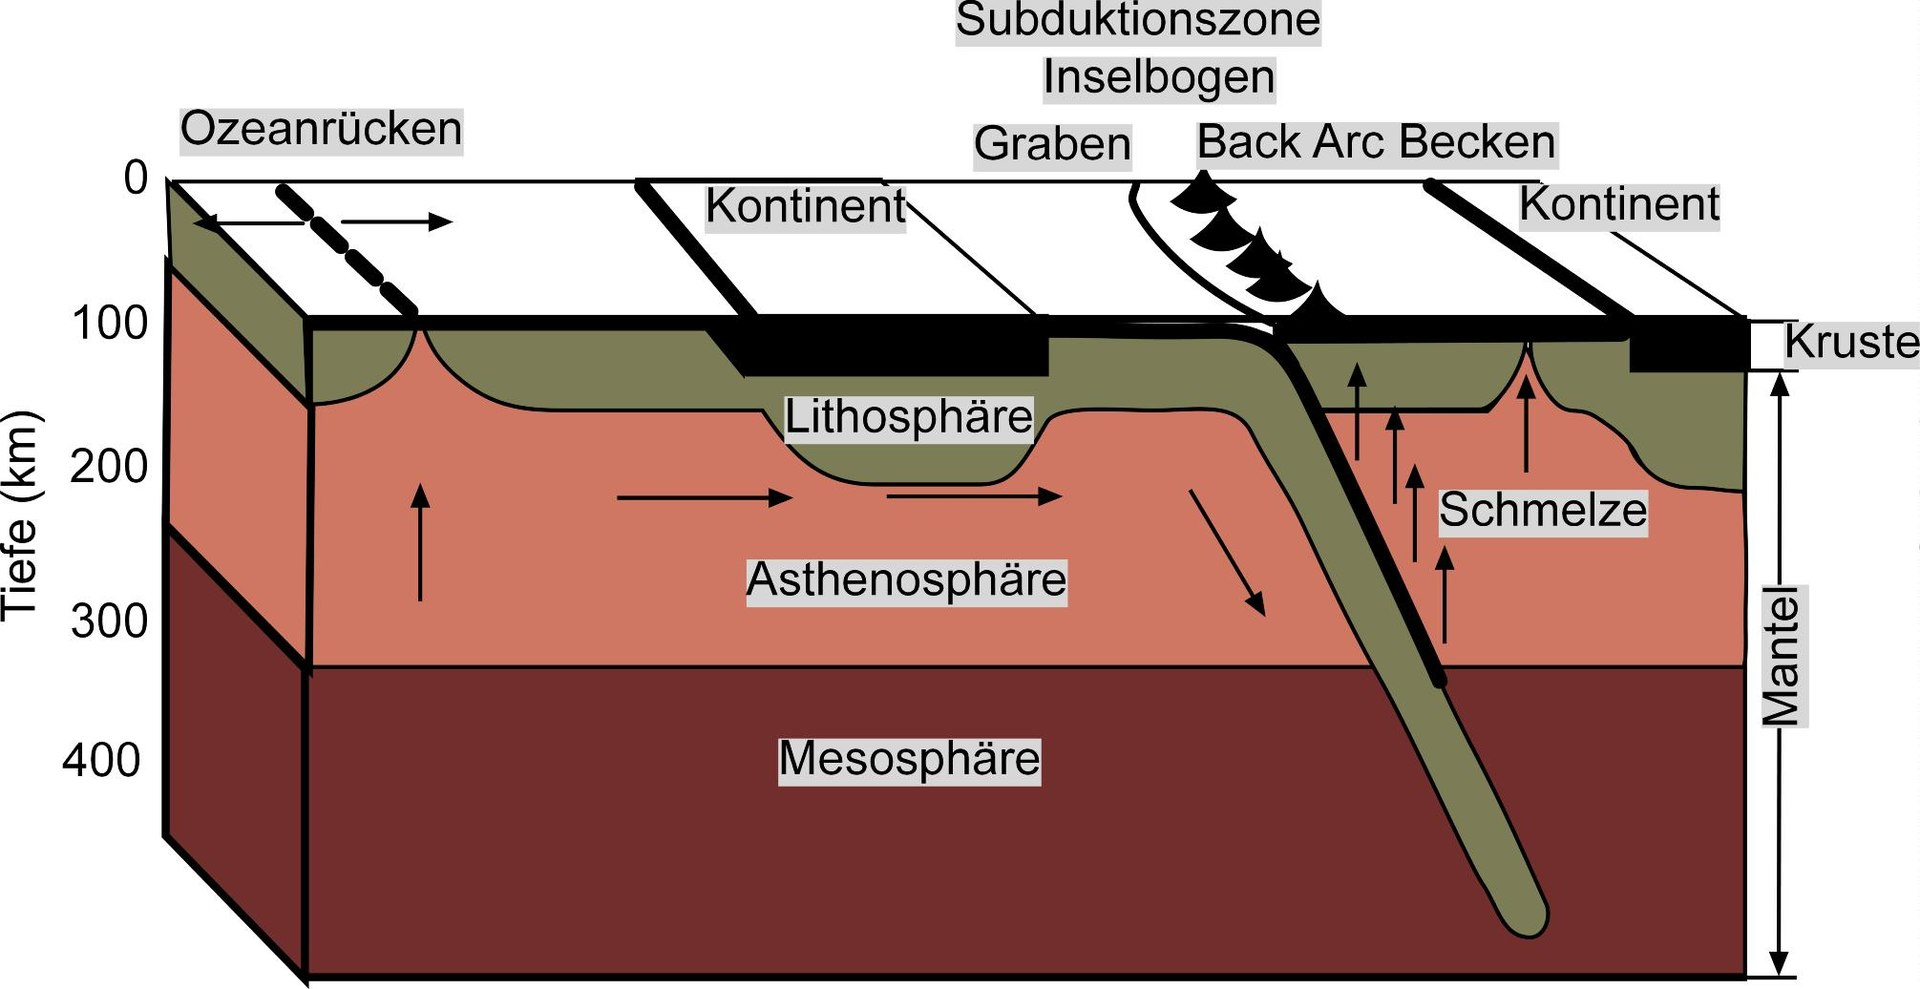
\includegraphics[width=0.9\textwidth]{Plattentekt.jpg}
    \caption{Schematische Darstellung der Dynamik von Lithosphärenplatten: Divergenz an Mittelozeanischen Rücken und Konvergenz an Subduktionszonen - [Gunnar Ries]}
\end{figure}

In einer Analyse von mehr als 35.000 weltweiten Katastrophenereignissen in den Jahren zwischen 1900 und 2015 des Karlsruher Institut für Technologie (KIT) zeigte sich, dass Erdbeben für 26\% der Schäden verantwortlich waren.
Der größte Schaden trat jedoch durch das Tohoku-Erdbeben am 11. März 2011 vor Honshū, Japan auf. Der Schaden durch das Erdbeben und dem dadurch ausgelösten Tsunami belief sich auf 18.500 Tote, 450.000 Menschen wurden obdachlos, und ein direkter wirtschaftlicher Schaden von etwa 296 Milliarden Euro. \cite{DANIELL}

Aufgrund des Erdbeben kam es zu der Fukushima-Nuklearkatastrophe im Atomkraftwerk Fukushima Daiichi.

Erdbebensicheres Design ist also von wirtschaftlicher und sicherheitstechnischer Bedeutung um die Aufgabe von Gebäuden zum Schutz des Menschen vor Naturereignissen und ein effektives Tragverhalten zu gewährleisten.

Die Ziele das Eurocode 8 sind daher das Schützen menschlichen Lebens, Schadensbegrenzung und das Aufrechthalten des Betriebs von Strukturen, die zum zivilen Schutz dienen wie zum Beispiel Krankenhäuser, die keine großen Schäden davontragen und den Betrieb nach dem Ereignis vortsetzen können sollen um ihren Aufgaben im Katastrophenschutz unmittelbar weiter nachzugehen.
Diese Anforderung der Wichtigkeit einer Struktur wird im Bedeutungsbeiwert erfasst. \cite{EC8}

\pagebreak

\section{Berechnung}
\label{sec:berechnung}

Grundlegend unterscheidet der Eurocode 8 vier verschiedene Berechnungsmethoden.

\begin{itemize}
  \item Vereinfachtes Antwortspektrenverfahren
  \item Antwortspektrenverfahren unter Berücksichtigung mehrerer Schwingungsformen (Modalanalyse)
  \item Kapazitätsspektrenmethode
  \item Zeitschrittberechnung
\end{itemize}

Da die beiden letzteren Verfahren ein genaueres Gebäudemodell vorraussetzen und deutlich aufwändiger sind als die Antwortspektrenverfahren eignen sich diese nur schwer für die Vordimensionierung von Strukturen. 
Hier werden weiterhin nur die vereinfachten Verfahren mittels Antwortspektren und Modalanalyse betrachtet, die Kapazitätsspektrenmethode und Zeitschrittberechnung soll aber kurz erläutert werden.

\subsection{Vereinfachtes Antwortspektrenverfahren}
\label{sec:Antwortspektrenverfahren}

Dieses Verfahren kann nur angewandt werden wenn die Anforderung aus dem Eurocode 8 an die Regelmäßigkeit des Grund- und Aufrisses erfüllt sind.
Hier wird nur die Grundschwingung der Struktur berücksichtigt. Daher kann dieses Verfahren nur angewendet werden wenn die höheren Schwingungsformen keinen wesentlichen Einfluss haben.

Die Grundschwingzeit kann in einer Näherung nach Müller/Keintzel bestimmt werden.

\begin{equation*}
T_1 = \frac{2 \pi H^2}{\alpha_1^2}\sqrt{\frac{m}{hEI}}
\end{equation*}

\thinspace

\begin{multicols}{2}
$H$: Gestamthöhe des Bauwerks \newline
$h$: Geschosshöhe \newline
$m$: Geschossmasse \newline
$EI$: Steifigkeit \newline 
$\alpha_1$: Schwingzeitbeiwert \newline
\columnbreak
\begin{flushright}
\begin{tabular}{ |c|c| } 
 \hline
 Geschosszahl & $\alpha_1$ \\
 \hline\hline
 1 & 1,32 \\ 
 2 & 1,53 \\ 
 5 & 1,71 \\ 
 10 & 1,78 \\ 
 \hline
\end{tabular}
\end{flushright}
\end{multicols}

Mit der Grundschwingzeit kann nun aus dem Antwortspektrum \cref{sec:Antwortspektren} der Bemessungswert der Spektralbeschleunigung $S_d$ bestimmt und die Gesamterdbebenkraft $F_b$ brechnet werden.

\begin{figure}[H]
    \centering
    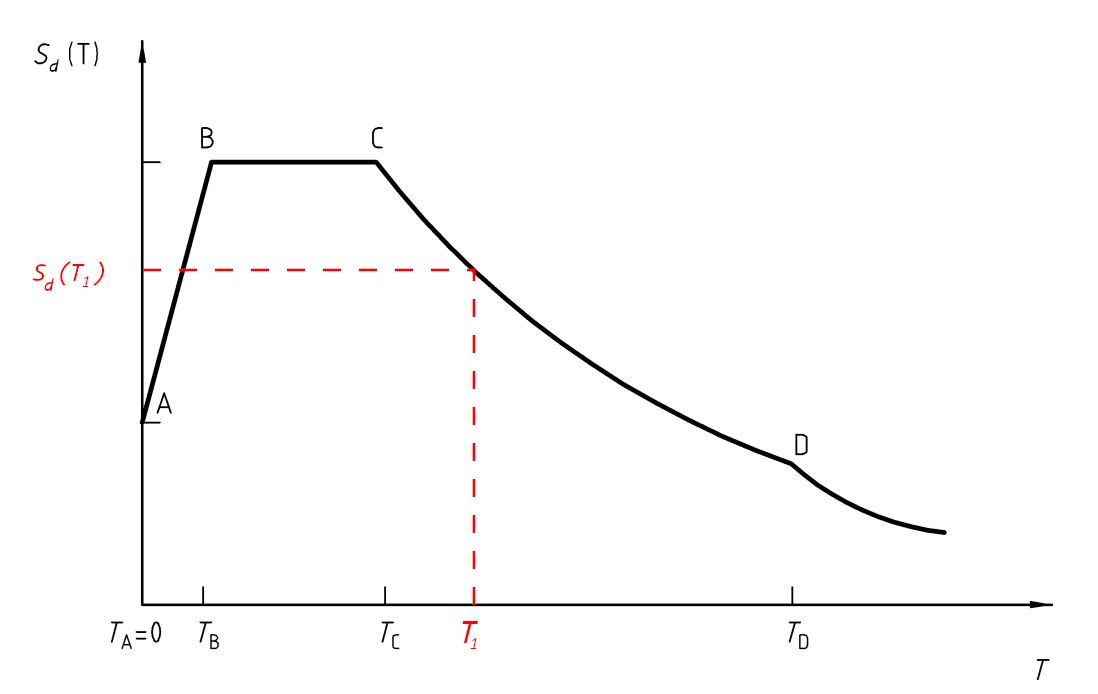
\includegraphics[width=0.9\textwidth]{AWS_Einleitung.png}
    \caption{Bemessungsspektrum}
\end{figure}

\begin{equation*}
F_b = S_d(T_1) \cdot M \cdot \lambda
\end{equation*}

Wobei $M$ die Gesamtmasse des Bauwerks und $\lambda$ der Korrekturfaktor von 0,85 für $T_1 \leq 2T_c$ für Gebäude mit mehr als zwei Geschossen und sonst $\lambda=1,0$ ist.
Die Grundschwingungsform darf linear angenährt werden. Somit können die angreifenden Horizontalkräfte vereinfacht linear über die Geschosse verteilt werden.

\begin{minipage}{0.55\textwidth}

\begin{equation*}
F_i = F_b \cdot \frac{z_i m_i}{\sum z_i m_i}
\end{equation*}

\vspace{2ex}
\vspace{2ex}

$F_i$: Am Geschoss $i$ angreifende Horizontalkraft \newline
$z_i$: Höhen vom Boden zu den Geschossen \newline
$m_i$: Geschossmassen \newline

\end{minipage}%
\hfill
\begin{minipage}{0.45\textwidth}

\begin{flushright}
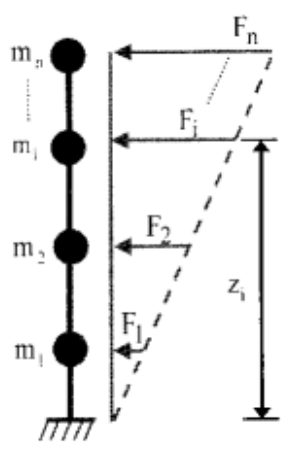
\includegraphics[width=0.4\linewidth]{Fi.png}
\end{flushright}

\end{minipage}%

Mit den Horizontalkräften können nun die Nachweise der Standsicherheit geführt werden.

\subsection{Antwortspektrenverfahren unter Berücksichtigung mehrerer Schwingungsformen (Modalanalyse)}
\label{sec:Modalanalyse}

Sind die Bedingungen an die Regelmäßigkeit des Bauwerks nicht erfüllt und es sollen mehr Schwingungsformen, zum Beispiel auch an einem dreidimensionalen Modell, betrachtet werden so kann eine Modalanalyse durchgeführt werden.

Das Vorgehen ist ähnlich zu \cref{sec:Antwortspektrenverfahren}, jedoch wird für jede Schwingungsform die Periode ermittelt, eine Spektralbeschleunigung bestimmt und die Horizontallasten anhand der Beteiligungsfaktoren der Schwingungsform angesetzt.

\begin{figure}[H]
    \centering
    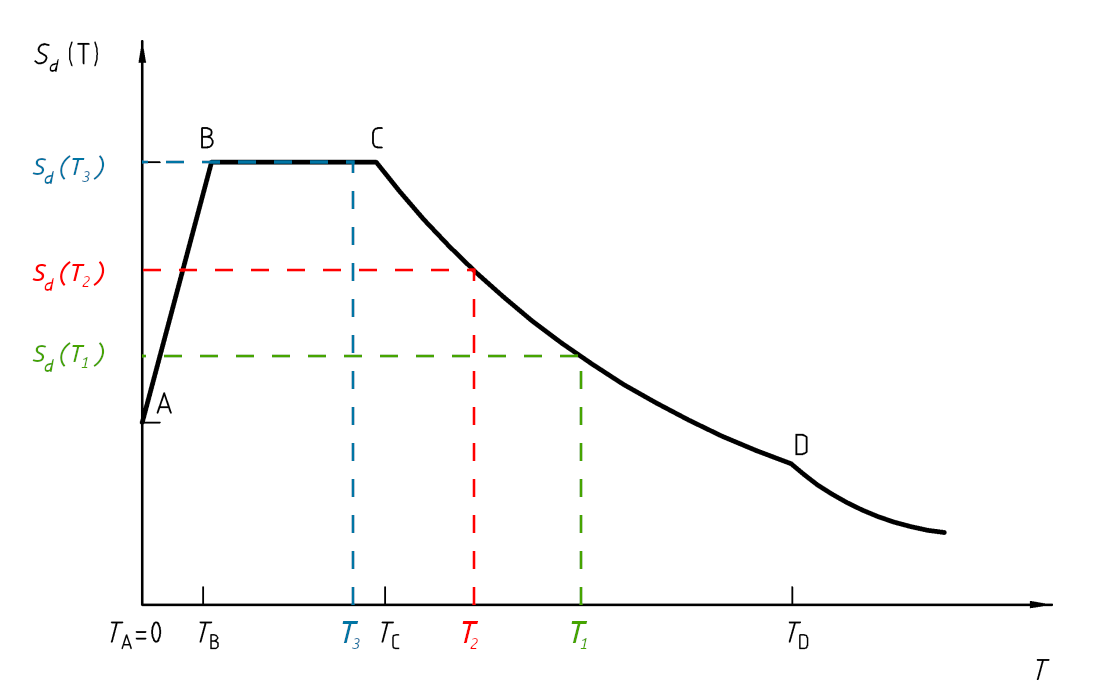
\includegraphics[width=0.9\textwidth]{AWS_Modal_Einleitung.png}
    \caption{Bemessungsspektrum}
\end{figure}

\begin{figure}[H]
    \centering
    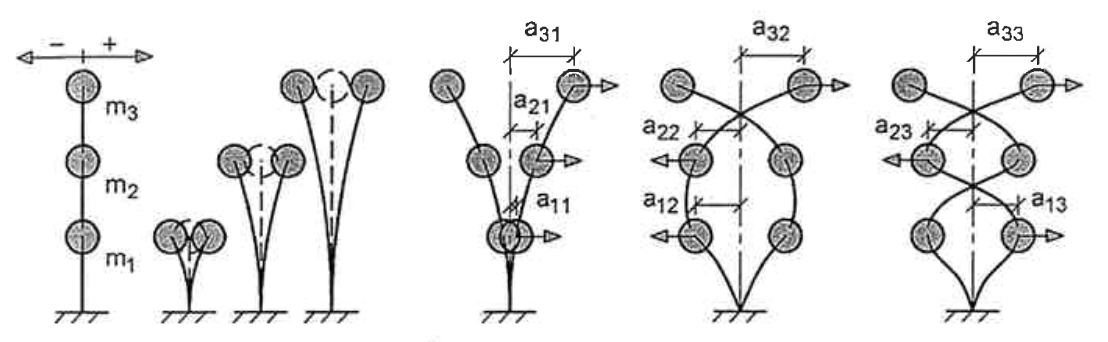
\includegraphics[width=0.9\textwidth]{Beteiligungsfaktoren.png}
    \caption{Eigenschwingungsformen eines Dreimassensystems \cite{Pocanschi}}
\end{figure}










Beteiligungsfaktoren





Anschließend müssen die modalen Schnittgrößen und Verschiebungen kombiniert werden. Hier sieht der Eurocode die SRSS-Methode (Square Root of Sum of Squares), die CQC-Methode (Complete Quadratic Combination) und die CQCi-Methode (CQC unter Berücksichtigung des Vorzeichens der i-ten Eigenform) vor.

\subsection{Kapazitätsspektrenmethode}
\label{sec:Kapazitaetsspektrenmethode}

Die auch als "pushover analysis" bezeichnete Methode ist ein nicht-elastisches statisches Verfahren unter Berücksichtung des Eigengewichts und monoton ansteigender horizontaler Lasten zur Bestimmung der Grenzlast über die Grenzduktilität.
Sie ist ein genaueres Verfahren zur Bestimmung der plastischen Kapizität, die in den vereinfachten Verfahren von dem Verhaltensbeiwert $q$ erfasst werden.

\subsection{Zeitschrittberechnung}
\label{sec:Zeitschrittberechnung}

Die Berechnung mittels Zeitschrittverfahren ("time-history analysis") ist eín nicht-lineares Verfahren, welches eine zeitabhängige Antwort einer Struktur über die direkte numerische Integration der Differentialgleichungen der Bewegung unter den im Eurocode 8 angegebenen Akzelerogrammen der Bodenbeschleunigung bestimmt. 

\pagebreak

\section{Erzeugung der Antwortspektren}
\label{sec:Antwortspektren}

\pagebreak

\section{Vordimensionierung}
\label{sec:vordimensionierung}

\pagebreak